% mnras_template.tex 
%
% LaTeX template for creating an MNRAS paper
%
% v3.0 released 14 May 2015
% (version numbers match those of mnras.cls)
%
% Copyright (C) Royal Astronomical Society 2015
% Authors:
% Keith T. Smith (Royal Astronomical Society)

% Change log
%
% v3.0 May 2015
%    Renamed to match the new package name
%    Version number matches mnras.cls
%    A few minor tweaks to wording
% v1.0 September 2013
%    Beta testing only - never publicly released
%    First version: a simple (ish) template for creating an MNRAS paper

%%%%%%%%%%%%%%%%%%%%%%%%%%%%%%%%%%%%%%%%%%%%%%%%%%
% Basic setup. Most papers should leave these options alone.
\documentclass[fleqn,usenatbib]{mnras}

% MNRAS is set in Times font. If you don't have this installed (most LaTeX
% installations will be fine) or prefer the old Computer Modern fonts, comment
% out the following line
\usepackage{newtxtext,newtxmath}
% Depending on your LaTeX fonts installation, you might get better results with one of these:
%\usepackage{mathptmx}
%\usepackage{txfonts}

% Use vector fonts, so it zooms properly in on-screen viewing software
% Don't change these lines unless you know what you are doing
\usepackage[T1]{fontenc}
\usepackage{ae,aecompl}


%%%%% AUTHORS - PLACE YOUR OWN PACKAGES HERE %%%%%
% Only include extra packages if you really need them. Common packages are:
\usepackage{graphicx}	% Including figure files
\usepackage{amsmath}	% Advanced maths commands
\usepackage{amssymb}	% Extra maths symbols

%%%%%%%%%%%%%%%%%%%%%%%%%%%%%%%%%%%%%%%%%%%%%%%%%%

%%%%% AUTHORS - PLACE YOUR OWN COMMANDS HERE %%%%%

\newcommand{\aw}[1]{\textcolor{red}{[AW: #1]}}
\newcommand{\hvp}[1]{\textcolor{green}{[HVP: #1]}}
\newcommand{\dm}[1]{\textcolor{magenta}{[DM: #1]}}


\newcommand{\popp}{\boldsymbol{\Psi}}
\newcommand{\objp}{\boldsymbol{\psi}}
\newcommand{\data}{\mathbf{d}}
\newcommand{\Teff}{T}
\newcommand{\logg}{g}
\newcommand{\pr}{\text{Pr}}
\newcommand{\de}{\text{d}}
\newcommand{\kpc}{\text{kpc}}


% Please keep new commands to a minimum, and use \newcommand not \def to avoid
% overwriting existing commands. Example:
%\newcommand{\pcm}{\,cm$^{-2}$}	% per cm-squared

%%%%%%%%%%%%%%%%%%%%%%%%%%%%%%%%%%%%%%%%%%%%%%%%%%

%%%%%%%%%%%%%%%%%%% TITLE PAGE %%%%%%%%%%%%%%%%%%%

% Title of the paper, and the short title which is used in the headers.
% Keep the title short and informative.
\title[Inferring properties of the White Dwarf population]{Inferring properties of the White Dwarf population of the Milky Way using astrometry and photometry}

% The list of authors, and the short list which is used in the headers.
% If you need two or more lines of authors, add an extra line using \newauthor
\author[A. Widmark]{
Axel Widmark$^1$\thanks{E-mail: axel.widmark@fysik.su.se} 
\\
% List of institutions
$^1$The Oskar Klein Centre for Cosmoparticle Physics, Department of
Physics, Stockholm University, AlbaNova, 10691 Stockholm, Sweden\\
}

% These dates will be filled out by the publisher
\date{Accepted XXX. Received YYY; in original form ZZZ}

% Enter the current year, for the copyright statements etc.
\pubyear{2018}

% Don't change these lines
\begin{document}
\label{firstpage}
\pagerange{\pageref{firstpage}--\pageref{lastpage}}
\maketitle

% Abstract of the paper
\begin{abstract}
The Gaia mission will provide precise astrometry for an unprecedented number of white dwarfs, for which there is enormous scientific potential. With such a large data set, it is possible to infer properties of the white dwarf population using only astrometric and photometric information. In this article we demonstrate how to do this using a mock data set with SDSS \emph{ugriz} photometry and astrometric information expected from future Gaia data releases.
We do so in the framework of a Bayesian Hierarchical Model, which is a powerful tool to infer properties of a stellar population while also taking into account all observational errors of individual stars. We demonstrate that astrometry significantly improves the statistical inference. We also show that the inference becomes more robust and less sensitive to systematic errors.
This is a powerful method to constrain stellar evolution, Type 1a supernovae progenitor scenarios, as well as the star formation history and dynamical history of the Milky Way.
\end{abstract}

% Select between one and six entries from the list of approved keywords.
% Don't make up new ones.
\begin{keywords}
white dwarfs -- stars: statistics -- astrometry
\end{keywords}

%%%%%%%%%%%%%%%%%%%%%%%%%%%%%%%%%%%%%%%%%%%%%%%%%%

%%%%%%%%%%%%%%%%% BODY OF PAPER %%%%%%%%%%%%%%%%%%







\section{Introduction}

The Sloan Digital Sky Survey (SDSS) catalogues a total number of $\sim 29,000$ spectroscopically confirmed white dwarfs \citep{2013ApJS..204....5K,2015MNRAS.446.4078K}. A fundamental difficulty in studying white dwarfs is that they have no fixed mass or size, such that their observational properties are largely degenerate with distance. This degeneracy can be broken with high quality spectrometry and accurate atmospheric models, although this is sensitive to systematic errors. The Gaia mission, soon to publish its second data release (DR2), is expected to increase the number of known white dwarfs by something like an order of magnitude \citep{2014A&A...565A..11C,Jordan:2006jg}. Gaia will also provide astrometric information for local neighbourhood white dwarfs, which previous astrometric missions were unable to do. Hipparcos had a limiting apparent magnitude of $V \sim 12.4$, while Gaia will see objects as dim as $V \sim 20$.

%White dwarfs are the eventual remnants of all light to intermediate mass stars. Upheld by electron degeneracy pressure and with no internal fusion, they are approximately Earth sized objects that cool over billions of years. A population of white dwarfs carries information about the star formation history and dynamical history of its environment. They also constrain models of stellar evolution and beyond Standard Model particle physics. White dwarfs are known to be SN1A thermonuclear supernovae progenitors, although the explosion mechanism is not known, which is something Milky Way white dwarf statistics could constrain.

With the enormous size of the Gaia data set, there is great potential in an approach that focuses on width rather than depth, by taking less detailed information into account but including a very large number of objects. In this article we demonstrate how to infer properties of the white dwarf population in the solar neighborhood, using SDSS \emph{ugriz} photometry and Gaia astrometry. We generate a mock data sample of white dwarfs from a population model of temperature, surface gravity and spatial number density distributions. All sample objects has photometry and parallax information with observational errors expected from SDSS and Gaia, and sample construction selection effects are taken into account. We retain the parameters of the population model using a Bayesian hierarchical model, which is a powerful tool to infer properties of a stellar population while also taking into account all observational errors of individual stars. We also show that small systematic errors in photometry or the assumed spatial number density distribution can give rise to large biases, but that these biases are quenched in the presence of Gaia astrometry.

We also discuss how to expand the statistical model when considering several different white dwarf populations with different properties. We consider the following divisions of the total white dwarf population into subpopulations: (i) White dwarfs form a family of phenomenological types, where the main classification is between DA and DB, depending on if the envelope is hydrogen or helium dominated. DA and DB stars can be identified with accurate photometry, as demonstrated by \cite{Mortlock:2008gf}. (ii) Disk and halo white dwarf populations are expected to have different properties. The halo population is older, and holds information about the Milky Way's distant past. (iii) Although very poorly constrained, a significant fraction of binary white dwarf systems are expected. We show that such a subpopulation can be identified with photometric and astrometric information alone.

This paper is organized as follows...



\section{Method}\label{sec:method}

The full posterior on both population parameters and object parameters is written

\begin{equation}\label{eq:fullposterior}
	\pr(\popp,\objp | \data ) = \pr(\popp)
    \prod_i \frac{S(\data_i) \pr(\data_i|\objp_i) \pr(\objp_i | \popp)}{\bar{N}(S,\popp)},
\end{equation}
where $\pr(\popp)$ is a prior on the population parameters; $S(\data_i)$ is the probability of being selected given the data of that object; $\pr(\data_i|\objp_i)$ is the likelihood of the data of an object given its object parameters; $\pr(\objp_i | \popp)$ is the probability of object parameters given the population parameters; finally, $\bar{N}(S,\popp)$ is the normalization to $\pr(\objp_i | \popp)$, and depends on the selection function and the population parameters.



\begin{table}
	\centering
	\caption{The 4 population parameters of our model, the 3 object parameters, and the data of the respective stars.}
	\label{tab:parameters}
    \begin{tabular}{l}
		\hline
		Population parameters, $\popp$ \\
		\hline
		$\alpha$,\quad $\bar{g}$,\quad $\sigma_g$,\quad $\gamma_g$ \\
        \hline
        Object parameters, $\objp_{i=1,...,n}$ \\
        \hline
        $\Teff$,\quad $\logg$,\quad $\Delta$ \\
        \hline
        Data, $\data_{i=1,...,n}$ \\
        \hline
        $\hat{\varpi}$,\quad $\sigma_{\hat{\varpi}}$,\quad $\hat{m}_{c=\{u,g,r,i,z\}}$,\quad $\sigma_{\hat{m}_c}$,\quad $l$,\quad $b$ \\
		\hline
	\end{tabular}
\end{table}

\subsection{Population model}\label{sec:populationmodel}

We list the population parameters of our model, encapsulated in a vector $\popp$, in table \ref{tab:parameters}, along with the object parameters and data. The population parameters are $\alpha$, which parameterizing the distribution of temperatures, and $\bar{g}$, $\sigma_g$, $\gamma_g$ which parameterize the distribution of surface gravities.

The distribution of surface gravity and effective temperature are parameterized by

\begin{equation}\label{eq:T&g}
\begin{split}
	\pr(\logg | \popp) & = t(\logg|\bar{g},\sigma_g,\gamma_g),\\
    \pr(\Teff | \popp) & = \exp (-\alpha \Teff),
\end{split}
\end{equation}
where $t(\logg)$ is the Student's t-distribution, with variance $\text{Var}(g) = \gamma_g^2 \sigma_g^2$. In this sense the quantity $\gamma_g$ parameterizes the heaviness of the tails of the t-distribution. The surface gravity $\logg$ is limited to the interval $(7,9.5)$. The temperature is limited to the interval $(1500,20000)$ K. In effect, this lower limit of 1500 K is not seen due to selection effects.

Also included in our model is a white dwarf number density function, expressed in terms of cylindrical coordinates $R$, $Z$ and $\Phi$,

\begin{equation}\label{eq:numberdensity}
\begin{split}
	n(\mathbf{x}) \propto
	\Bigg[ 
		& \exp\Bigg(-\frac{R}{L_\text{thin}}\Bigg)\exp\Bigg(-\frac{|Z|}{H_\text{thin}}\Bigg) \\
		& +f_\text{thick}\exp\Bigg(-\frac{R}{L_\text{thick}}\Bigg)\exp\Bigg(-\frac{|Z|}{H_\text{thick}}\Bigg) \\
		& +f_\text{halo}\Bigg( \frac{(R^2+Z^2/q_\text{halo}^2+R_\text{core}^2)^{1/2}}{L_\text{halo}}^{-\eta_\text{halo}} \Bigg),
	\Bigg]
\end{split}
\end{equation}
where $f_\text{thick}=0.06$, $f_\text{halo}=6\times10^{-5}$, $L_\text{thin}=L_\text{thick}=3.5~\kpc$, $L_\text{halo}=8.5~\kpc$, $R_\text{core}=1~\kpc$, $H_\text{thin}=0.26~\kpc$, $H_\text{thick}=1~\kpc$, $q_\text{halo}=0.64$ and $\eta_\text{halo} = 2$. Assuming a solar position of $R_\odot=8~\kpc$ (where the height of the Sun above the plane is neglected), the galactic coordinates are given by heliocentric coordinates through

\begin{equation}
\begin{split}
	& R(d,l,b) = [d^2\cos^2b-2 R_\odot d \cos^2b\cos^2+R_\odot^2]^{1/2}, \\
	& Z(d,l,b) = d \sin b.
\end{split}
\end{equation}
The azimuthal angle can be neglected, as the galaxy is assumed to be axisymmetric in this model.

\aw{Population parameter prior should probably be written here}







\subsection{Data and likelihood}\label{sec:data}

The data of each respective white dwarf is listed in table \ref{tab:parameters}. A hatted quantity ($\hat{\varpi}$) refers to an observed value of some measurement error, while a non-hatted quantity ($\varpi$) refers to an observable's true value. The data of a white dwarf consists of parallax measurement $\hat{\varpi}$ and error $\sigma_{\hat{\varpi}}$, apparent magnitude in five bands $\hat{m}_{c=\{u,g,r,i,z\}}$ with their respective errors $\sigma_{\hat{m}_c}$, and finally the angular position on the sky $\{l,b\}$. The angles $l$ and $b$ are written without hats, to signify that they are taken at face values, as the errors are small and can be neglected.

The likelihood of an $i$th object is

\begin{equation}\label{eq:likelihood}
	\pr(\data_i | \objp_i) = \mathcal{N}(\varpi(\objp_i)|\hat{\varpi},\sigma_{\hat{\varpi}})\prod_{c} \mathcal{N}(m_c(\objp_i)|\hat{m}_c,\sigma_{\hat{m}_c}),
\end{equation}
where the color bands iterated over in the product are $c = \{u,g,r,i,z\}$, and $\mathcal{N}(x | \mu,\sigma)$ is the normal distribution of mean $\mu$ and standard deviation $\sigma$. The factor containing parallax information is dropped when no parallax information is present.

The magnitudes $m_c(\objp_i)$ are functions of the object parameters. Absolute magnitudes $M_c$ in the \emph{ugriz} color bands come from the atmospheric models of Bergeron, as functions of effective temperature $\Teff$ and surface gravity $\logg$.








\subsection{Object parameters}\label{sec:objectparams}

Each white dwarf has a set of object parameters encapsulated in $\objp_i$, as listed in table \ref{tab:parameters}. It consists of the effective temperature $\Teff$, the surface gravity $\logg$, and $\Delta$ which parameterizes the distance.

Conceptually, the most straight forward parameterization would be to have the distance $d$ as the third object parameter. However, this creates some sampling difficulties coming from the fact that $\logg$ and $d$ are heavily degenerate, which is problematic especially when there is no parallax information that constrains the distance. This is illustrated in figure \ref{fig:banana}. Therefore the distance is parameterized in terms of $\Delta$, which is the relative change to the ideal distance given $\Teff$ and $\logg$. Let $\tilde{d}(\Teff,\logg)$ be the distance that maximizes the color factor of the likelihood function, like

\begin{equation}
	\tilde{d} = 
    h^{-1}\left( \frac{\sum_c \sigma_{\hat{m}_c}^{-2} (\hat{m}_c-M_c(\Teff,\logg))}{\sum_c \sigma_{\hat{m}_c}^{-2}} \right),
\end{equation}
where $h^{-1}$ is the inverse of $h(d)=5[\log_{10}(d/\text{pc})-1]$, which is the difference between apparent to absolute magnitude. The distance parameterized by the object parameters is then $d=\Delta\tilde{d}(\Teff,\logg)$. It is crucial to account for the Jacobian factor that arises with this parameterization, which is $\de \Teff\, \de \logg\, \de d = \de \Teff\, \de \logg\, \de \Delta\, \tilde{d}(\Teff,\logg)$.

\begin{figure}
	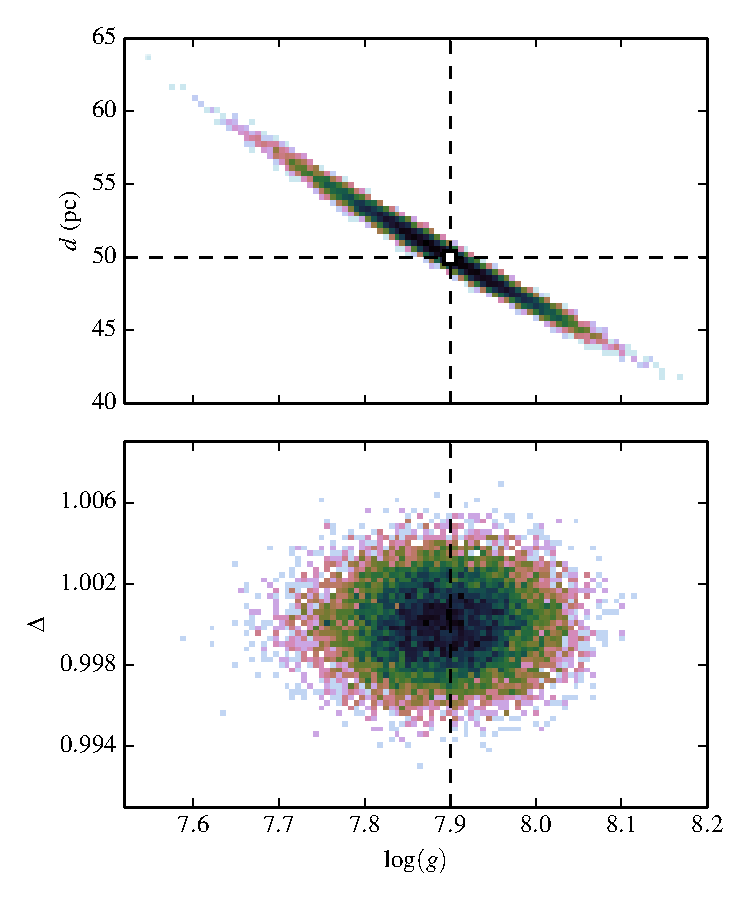
\includegraphics[width=\columnwidth]{banana.pdf}
    \caption{A posterior density of an object with true parameters $\Teff=20000$ K, $\logg=8$, and $d=50$ pc, with photometric errors of $\sigma_{\hat{m}_c}=0.03$ in all \emph{ugriz} color bands. The population parameters are set to $\alpha=3.5$, $\bar{g}=8$, $\sigma_g=0.1$, and $\gamma_g=1.2$. Because the photometric errors are somewhat large, the constraint to the surface gravity is mostly due to the prior set by the population model. The top panel shows the posterior density over $\logg$ and $\Delta$, while the bottom panel shows the same posterior in a $\logg$ and $d$ parameterization. This illustrates the degeneracy between surface gravity $\logg$ and distance $d$, which can be problematic for a Metropolis-Hastings algorithm to sample.}
    \label{fig:banana}
\end{figure}







\subsection{Object posterior}\label{sec:objectposterior}

The posterior on a specific object also includes the term $\pr(\objp_i | \popp)$, normalized by the quantity $\bar{N}(S,\popp)$. It is given by the population, parameterized by the population parameters $\popp$.

\begin{equation}
\begin{split}
	& \pr(\objp_i | \popp) \de \Teff \de \logg \de d  \\ & \propto
    d^2 n(l,b,\varpi) \pr(\Teff | \popp) \pr(g | \popp) \de \Teff \de \logg \de d \\
    & = \Delta^2\tilde{d}^3(\Teff,\logg) n(l,b,\varpi) \pr(\Teff | \popp) \pr(g | \popp) \de \Teff \de \logg \de \Delta,
\end{split}
\end{equation}
where $n$ is the number density of white dwarfs as a function of spatial position (possible here to also include velocity, but will leave that for now). It is implicit in this expression that the true parallax $\varpi$ is a function of the object parameters $\objp_i$.

The normalization factor is given by

\begin{equation}\label{eq:normalization}
	\bar{N}(S,\popp) = \int \de\Teff\, \de \logg\, \de^3\mathbf{x}\,
    \pr(\Teff | \popp) \pr(\logg | \popp) \pr(\mathbf{x} | \popp) S(\Teff,\logg,\mathbf{x}),
\end{equation}
basically an integral over the possible properties of a hypothetical white dwarf drawn from the population model, times the probability of being selected. The probability of being selected is the probability of being included in the sample, given by the cuts on observables and an object's intrinsic properties. This is formulated later in equation \eqref{eq:selection}. If the sample is incomplete, such a factor should also be included in the selection function, although we do not consider such effects here.



\section{Mock data and inference}\label{sec:mock}

To test the algorithm, mock data is generated from a population model, with population parameters $\alpha=3.5$, $\bar{g}=7.9$, $\sigma_g=0.1$, and $\gamma_g=1.2$, and the white dwarf number density $n(\mathbf{x})$ as described in section \ref{sec:populationmodel}. We compare the case of having no astrometric information, versus having parallax measurements with the precision expected from Gaia DR2.

\subsection{Sample cuts}

We define a sample by making cuts on observable properties, either on actual data or in our case on mock data of a generated catalogue. Depending on the errors of these observables, these cuts correspond more or less well to cuts in the objects' intrinsic properties. In this case we make cuts on apparent magnitude and color. We do not make a volume limited sample by making cuts on parallax -- we want to compare to the case when astrometry is not available, hence we need to construct the sample without such information. The cut in observed color is made such that we put an upper limit to the temperature of white dwarfs included in our sample. The limit in apparent magnitude sets a maximum distance for a white dwarf, as a function of temperature, where the hottest objects are seen to furthest distance.

There are several reasons for not allowing very high temperatures in our samples (although the exact limit is rather arbitrary). Very hot objects are also very rare, but because they are seen to much further distance they are still numerous. How many are seen depends on the properties of the population, but this is degenerate with the assumed spatial distribution and the distribution of dust. Furthermore, with high enough temperature the peak of the objects spectrum is actually of shorter wavelength than the $u$ band, in which case the inference on an objects temperature becomes very weak. When working with actual data, it is also necessary to identify what objects are white dwarfs and what objects are not. With a very hot, far away objects this is difficult, especially since the distance will be poorly constrained. These issues can be circumvented with good parallax measurements, enabling the construction of a volume limited sample.

We make the following cut in color, demanding that

\begin{equation}
	\hat{\delta}_{ugr} \equiv 0.27\hat{m}_u+0.23\hat{m}_g-0.5\hat{m}_r>-0.183.
\end{equation}
Without measurement errors, this cut corresponds to limiting the white dwarf temperature to $\Teff<20,000$ K. This is illustrated in figure \ref{fig:colors_cut}.

\begin{figure}
	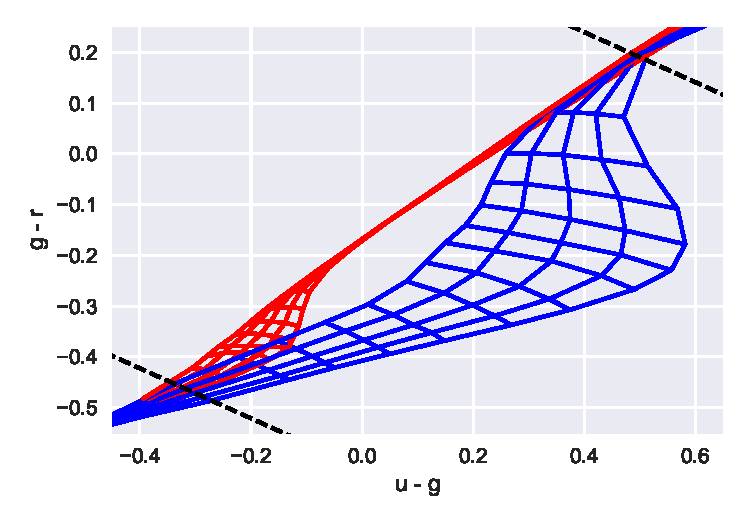
\includegraphics[width=\columnwidth]{colors_cut.pdf}
    \caption{Colors of a DA white dwarf, in lines of constant $\Teff$ or $\logg$. The black dashed line corresponds to the color cut in $\hat{\delta}_{ugr}$, where objects to the upper right are included in our sample, while objects to the lower left are excluded.}
    \label{fig:colors_cut}
\end{figure}

We also make a cut in brightness, by demanding that the Gaia $G$ band apparent magnitude fulfills that

\begin{equation}
	\hat{m}_G < 18.
\end{equation}
The brightness is done in the Gaia $G$ band, as the parallax errors is correlated to this observable. The errors on the $m_G$ are expected to be very small, and assumed to be $\sigma_{\hat{m}_G}=0.001$, also in terms of systematic errors as the passband is very broad. In principle, this criteria could equally well have been formulated in terms of some combination of the $ugriz$ apparent magnitudes.

Given these cuts to observables, the selection function is written

\begin{equation}\label{eq:selection}
\begin{split}
	S(\Teff,\logg,\mathbf{x}) = 
    	      & \int \de \hat{m}_G \Theta \big( 18-\hat{m}_G \big)\mathcal{N}\big( \hat{m}_G | m_G,\sigma_{\hat{m}_G} \big) \\
    \times & \int \de \hat{\delta}_{ugr} \Theta \big( \hat{\delta}_{ugr}+0.183 \big) \mathcal{N}\big( \hat{\delta}_{ugr} | \delta_{ugr},\sigma_{\hat{\delta}_{ugr}}\big),
\end{split}
\end{equation}
where the error on $\hat{\delta}_{ugr}$ is given by

\begin{equation}
	\sigma_{\hat{\delta}_{ugr}} = \sqrt{ 0.27 \sigma_{\hat{m}_u}^2 + 0.23 \sigma_{\hat{m}_g}^2 + 0.5 \sigma_{\hat{m}_r}^2 },
\end{equation}
assuming that the different color band errors are uncorrelated.


\subsection{Generating a mock data catalogue}

The errors in photometric magnitude vary with apparent magnitude. In order to account for this effect and have realistic errors for our mock data set, we set the errors of our object to the median errors of SDSS DR9, in bins of observed apparent magnitude of width 0.5 mag. This is visible in figure \ref{fig:magnitude_error}. We limit the minimum \emph{ugriz} magnitude error to 0.01, in order to account for possible systematic errors.

\begin{figure}
	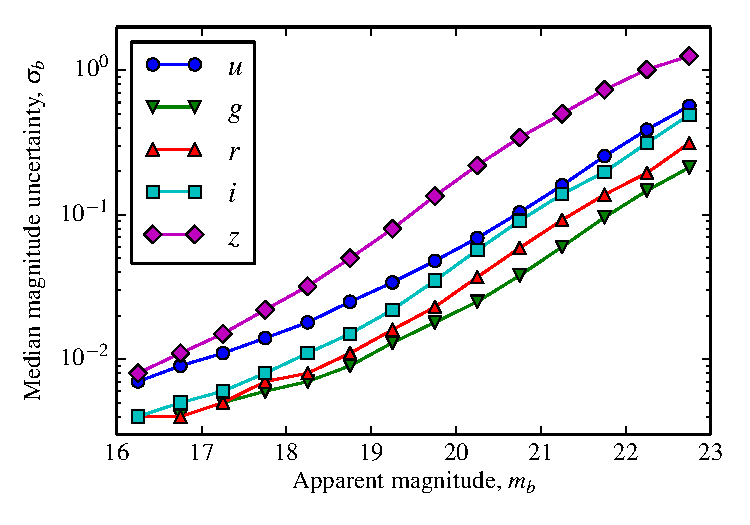
\includegraphics[width=\columnwidth]{median_app_errors.pdf}
    \caption{The median magnitude errors in SDSS DR9, as a function of observed apparent magnitude.}
    \label{fig:magnitude_error}
\end{figure}

Gaia DR2 will have a limiting magnitude of $G=21$, with parallax uncertainties smaller than $0.04$ mas for sources with $G<15$, about $0.1$ mas for sources with $G=17$, and about $0.7$ mas at $G=20$.\footnote{https://www.cosmos.esa.int/web/gaia/dr2} In order to account for this magnitude dependence, we interpolate these points according to figure \ref{fig:parallax_error}.

\begin{figure}
	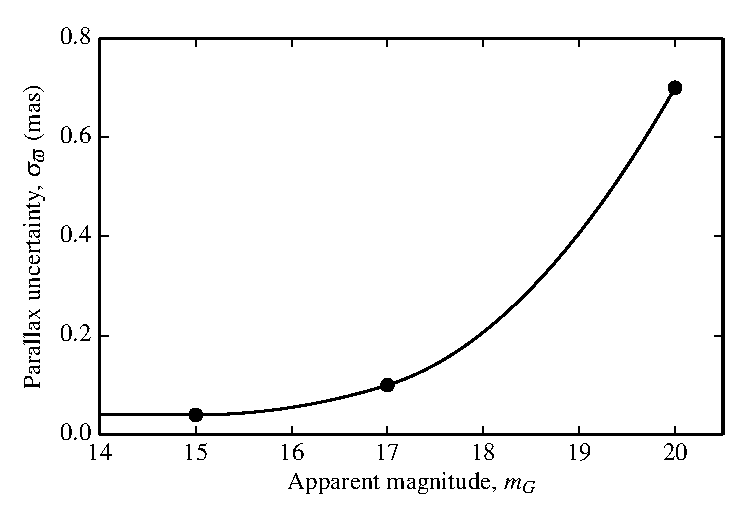
\includegraphics[width=\columnwidth]{parallax_error.pdf}
    \caption{Parallax error as a function of $G$ magnitude. The dots correspond to magnitudes $G=15,17,20$. For $G\leq 15$ the parallax error is 0.04 mas and constant.}
    \label{fig:parallax_error}
\end{figure}

The mock catalogue is generated by rejection sampling. An object is drawn randomly from the true population model: the object parameters $\Teff$ and $\logg$ are distributed as described in \eqref{eq:T&g} and can be randomized analytically; the position is distributed according to $n(\mathbf{x})$ and can be randomized by rejection sampling, knowing that there is a maximal distance a white dwarf can have to be included in our sample (observational errors included). A randomly drawn object is then given observable quantities with errors as described above. If the object observables fulfill the selection cuts, the object is included in the sample; if not, it is rejected.

In this article, we construct a sample with 10,000 DA white dwarfs. The distribution of true parameter values is visible in figure \ref{fig:10000WDs}. In this figure, selection effects are manifest. The maximum distance is clearly seen as a function of temperature (and surface gravity, to lesser extent) in the bottom panel. Even though cool stars are much more numerous in terms of spatial number density, it is actually hot stars near 20,000 K that dominate our sample, as they are seen to further distance. Very far away white dwarfs have low apparent luminosity and hence large color errors; this gives some scatter in the selection function such that the upper limit on temperature is blurred. The hottest object in this sample has an effective temperature of $\Teff=28,240$ K, and is located at a distance of 1.22 kpc. The two most distant objects are located at 1.27 kpc, and has surface gravities of $\logg=7.82$ and $\logg=7.71$, which is illustrative of the fact that lower surface white dwarfs are brighter and therefore seen to further distance. The lowest temperature white dwarf of our sample has a temperature of 1717 K.

Our sample size of 10,000 DA white dwarfs is a reasonable number of white dwarfs given the cuts BLABLA

\begin{figure}
	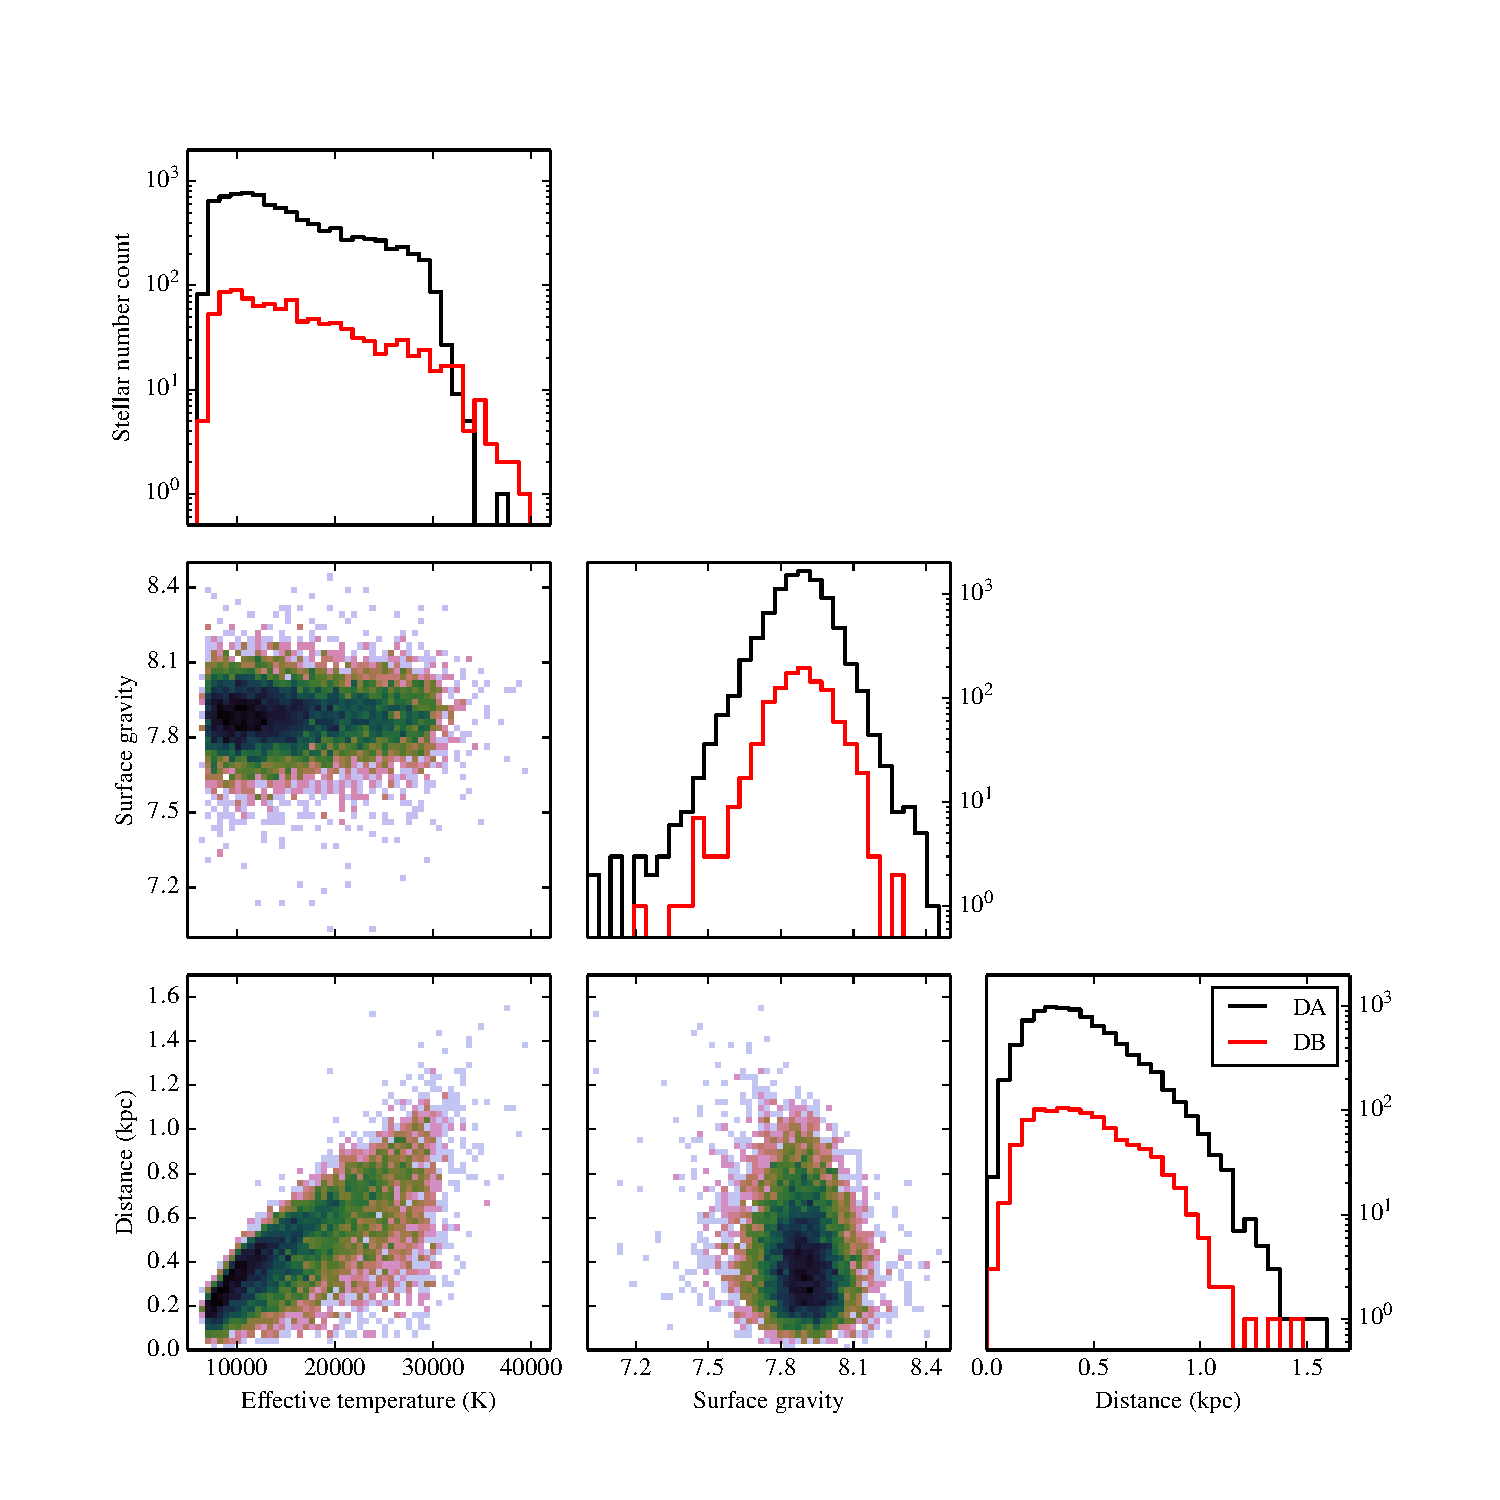
\includegraphics[width=\columnwidth]{10000WDs.pdf}
    \caption{The temperature, surface gravity and distance of our mock data sample. The horizontal axis, denoting temperature, is shared between the two panels. For visibility, only 2,000 objects are included in this figure.}
    \label{fig:10000WDs}
\end{figure}





\subsection{Results}

RUN CHAIN WITH BURN-IN AND YADA YADA

The inferred posterior distributions are visible in figures \ref{fig:chain} and \ref{fig:chain_parallax}, where the former has no parallax information.

\begin{figure*}
	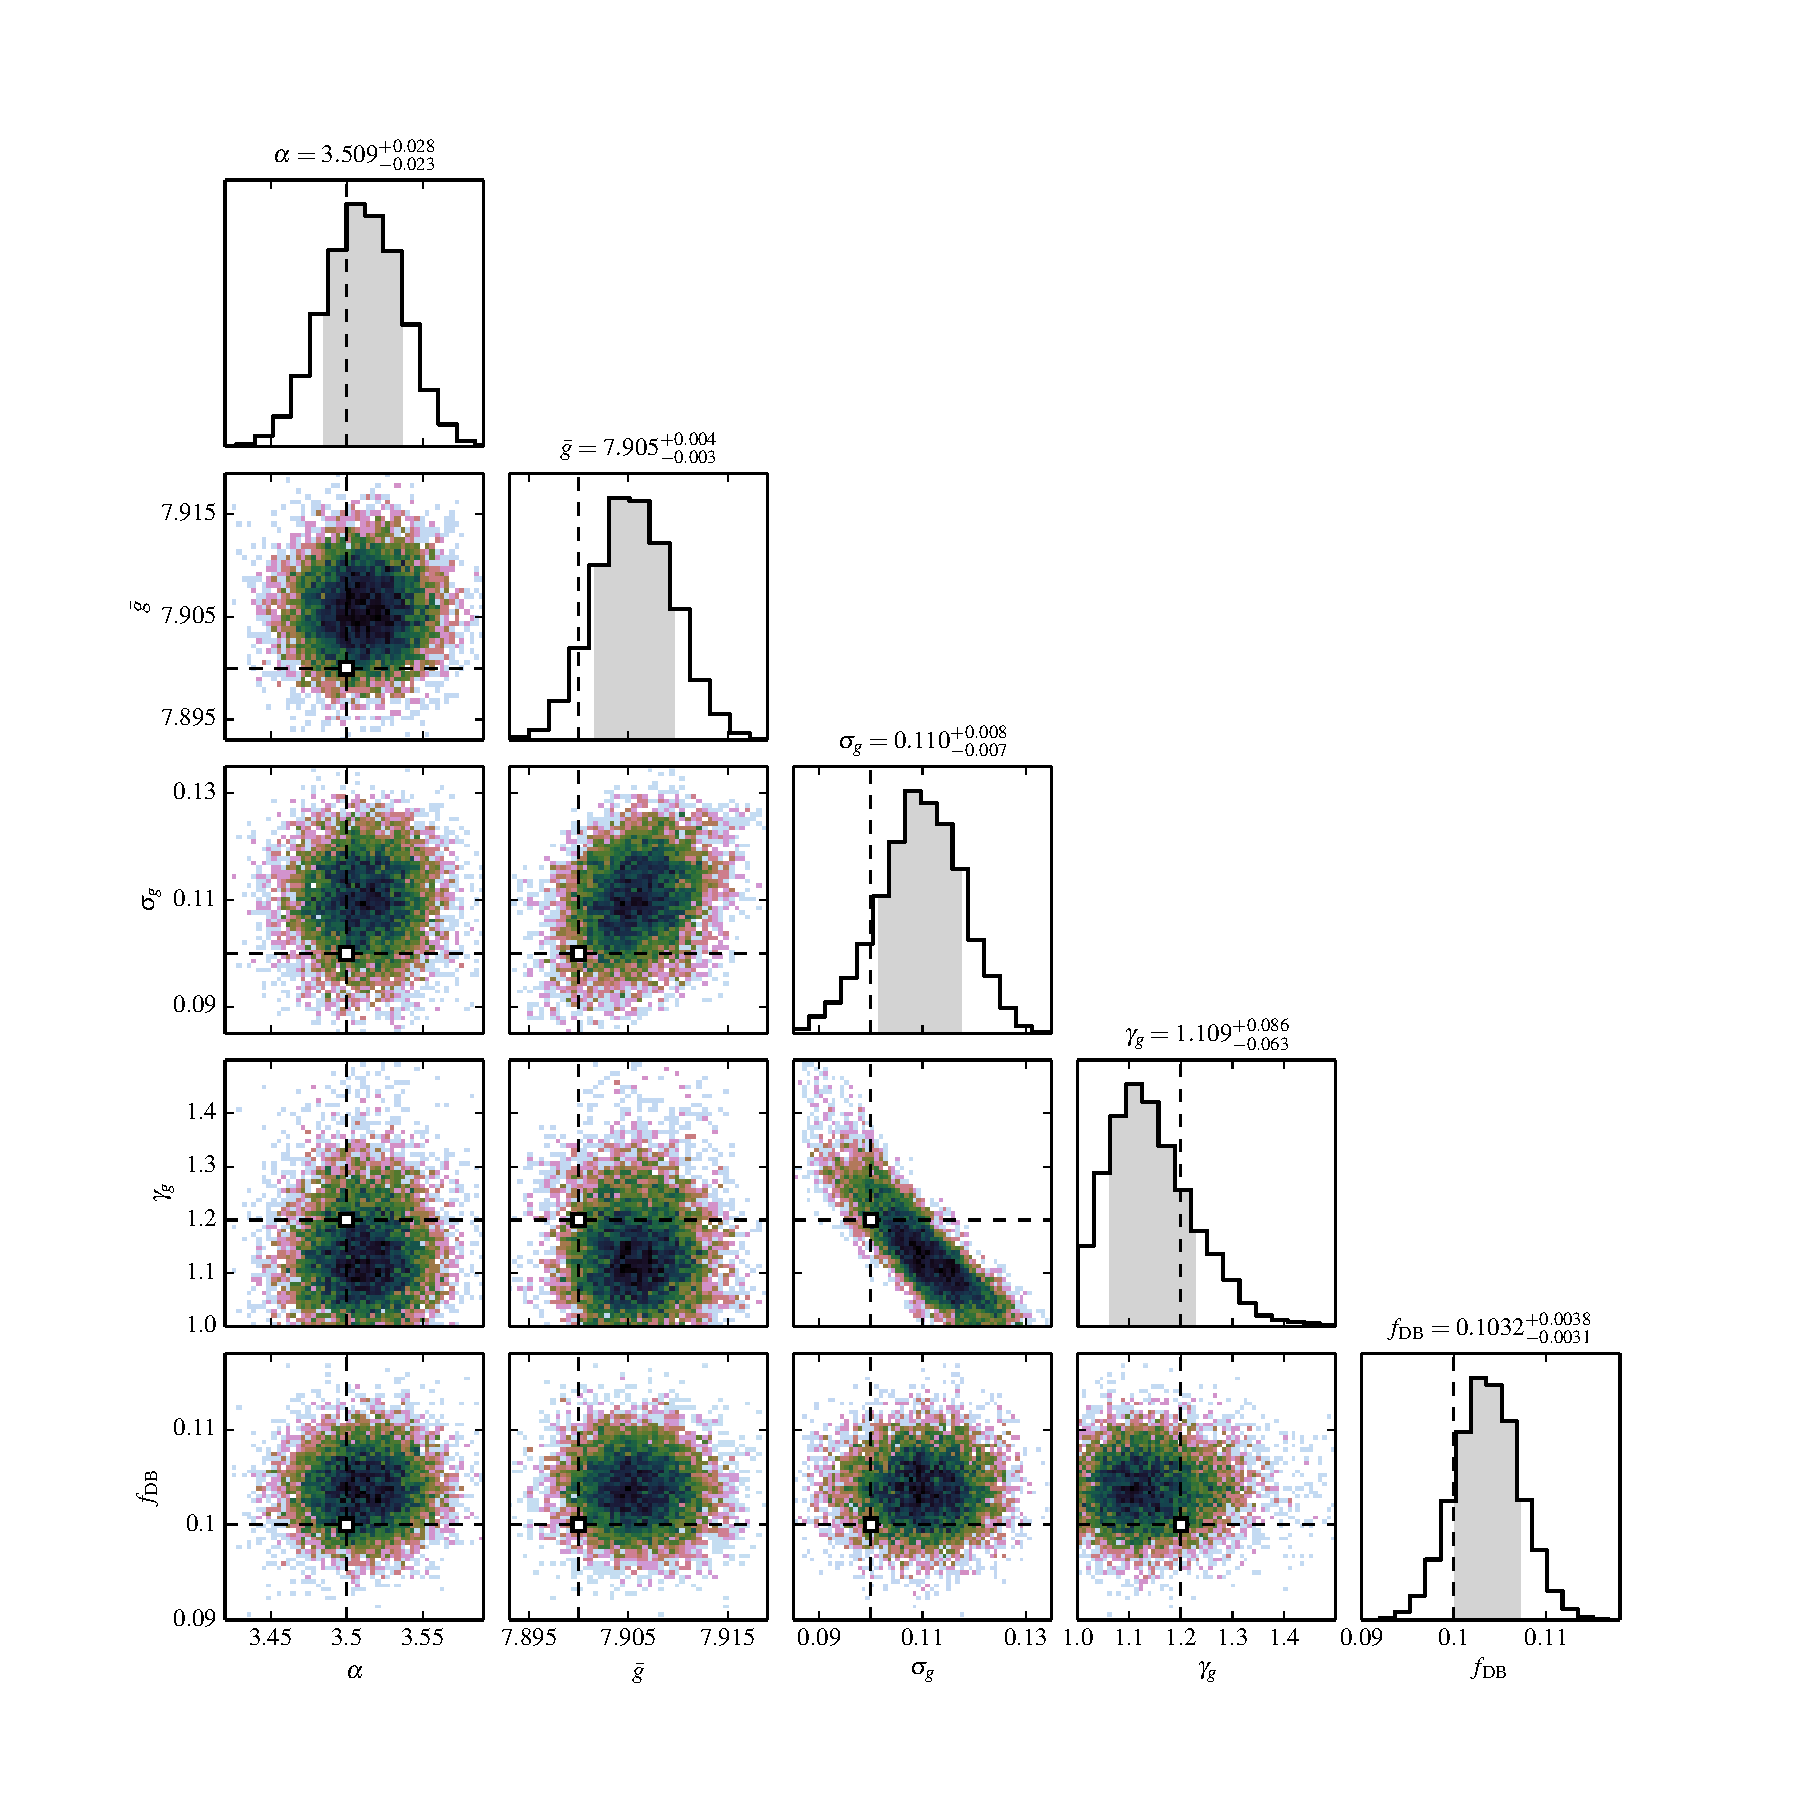
\includegraphics[width=.8\textwidth]{toy_chain.pdf}
    \caption{Posterior density of the population parameters, for a mock data set with no astrometric information.}
    \label{fig:chain}
\end{figure*}

\begin{figure*}
	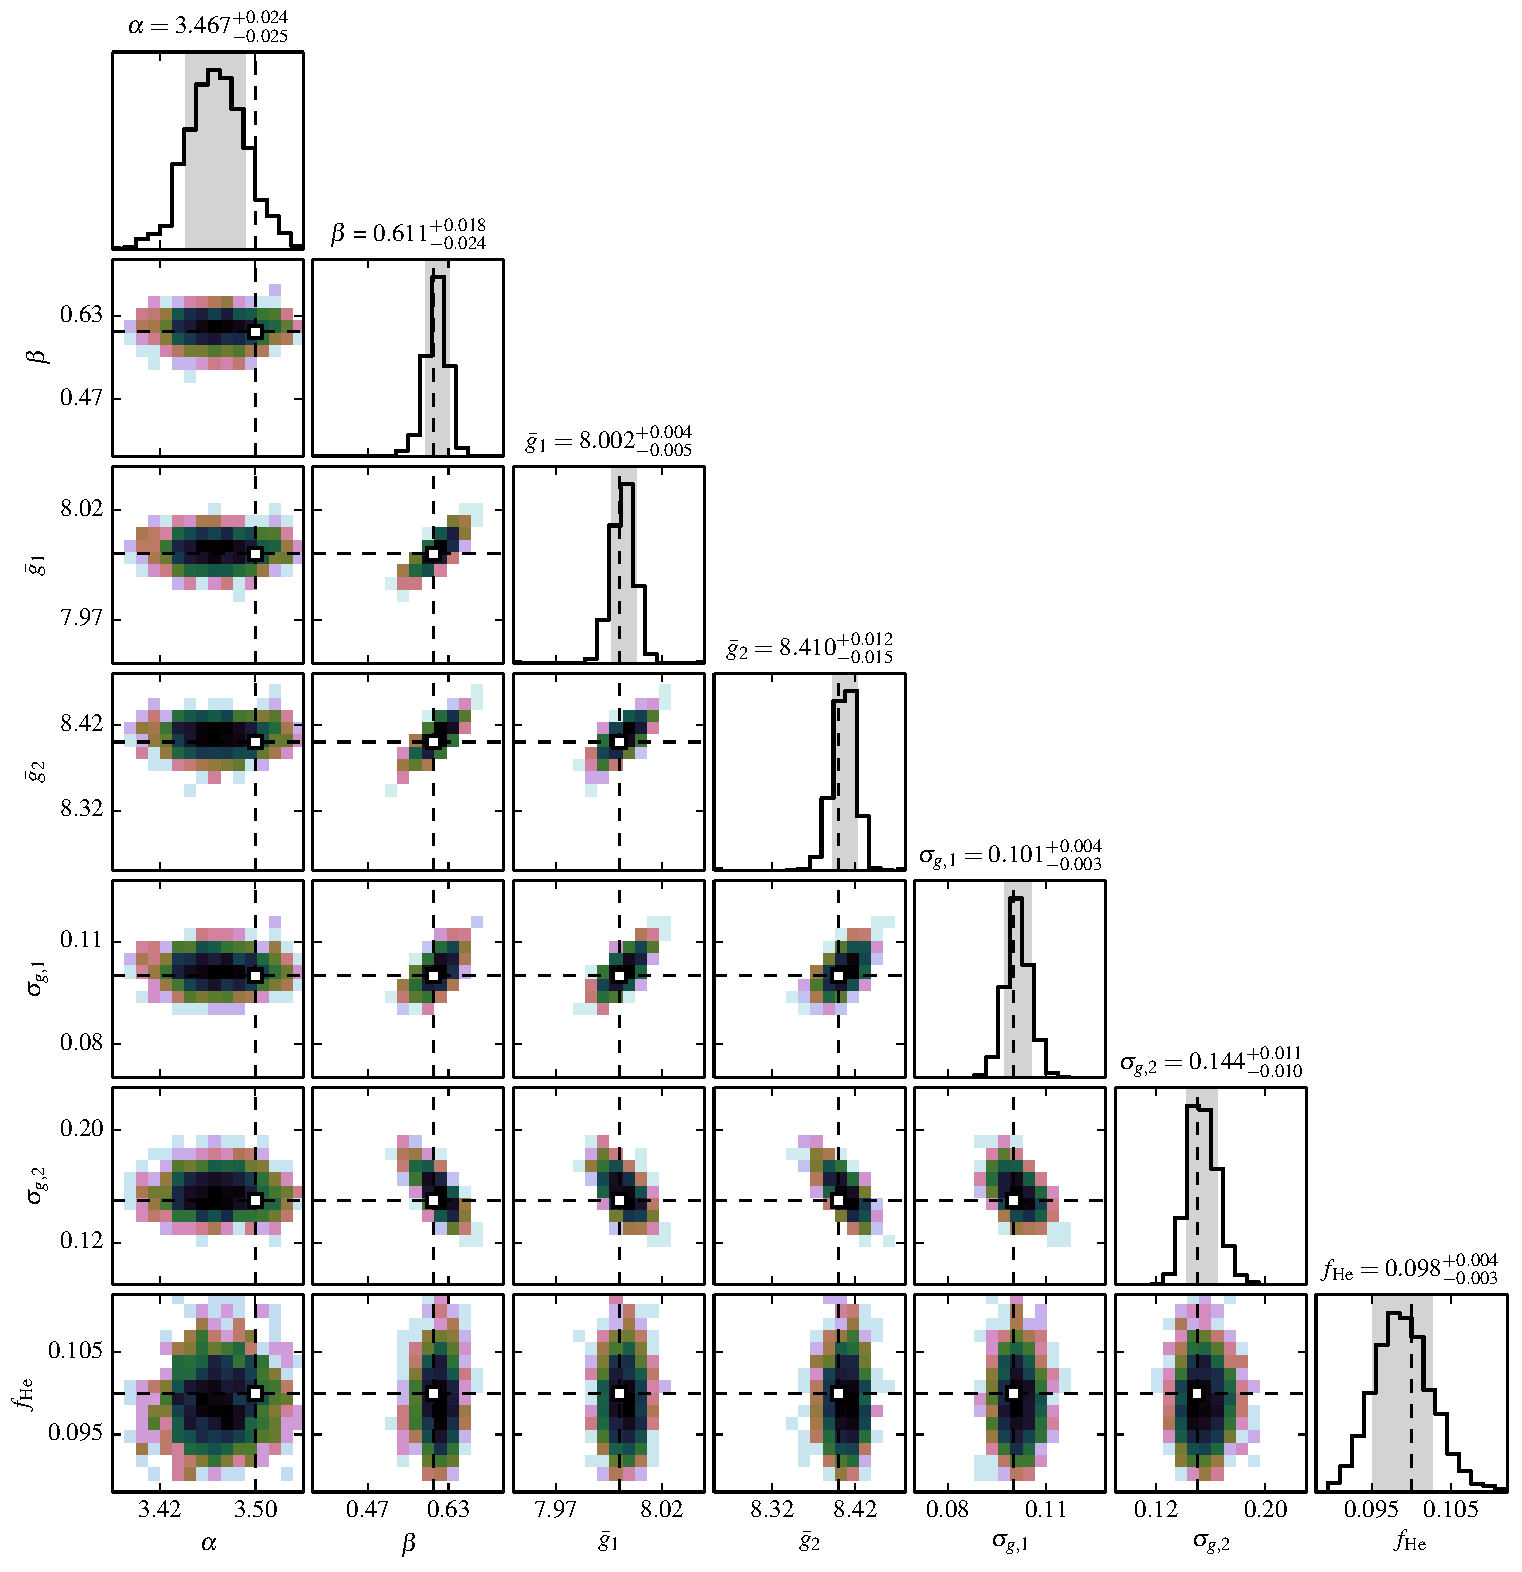
\includegraphics[width=.8\textwidth]{toy_chain_include-parallax.pdf}
    \caption{Posterior density of the population parameters, for a mock data set with parallax information.}
    \label{fig:chain_parallax}
\end{figure*}










\section{White dwarf subpopulations}

The actual population of white dwarfs in the Milky Way is of course much richer and complicated than the model described above. We only have white dwarfs of the hydrogen rich type (DA), while in reality there is something like 10 \% helium rich (DB) white dwarfs. Furthermore, younger white dwarfs are more abundant within the disk, while older white dwarfs have had more time to migrate into the halo.

In the case of several distinct populations, the total population is no longer described by a single set of population parameters $\popp$.






\subsection{DA and DB populations}

Hydrogen rich and helium rich white dwarfs, known as DA and DB, have different spectra and emission lines. This translates into somewhat different colors for DA and DB, such that they are differentiable from eachother with multiband photometry of sufficient precision. In order to account for both DA and DB populations, one can add the fraction of DB white dwarfs ($f_\text{DB}$) to the population paremeters $\popp$. In such a case we would add a labelling object parameter $X_i = \{\text{DA},\text{DB}\}$ to each object.

In the statistical model, as summarized in equation \eqref{eq:fullposterior}, we would replace the term

\begin{equation}
\begin{split}
	& \pr(\data_i | \objp_i) \pr(\objp_i | \popp)
	\rightarrow \\
	\Big[
	(1-f_\text{DB}) & \pr(\data_i | \objp_i,X_i=\text{DA}) \pr(\objp_i | \popp) + \\
	+ f_\text{DB} & \pr(\data_i | \objp_i,X_i=\text{DB}) \pr(\objp_i | \popp)
	\Big].
\end{split}
\end{equation}
Also the normalization term $\bar{N}$, as seen in equation \eqref{eq:normalization}, is changed by replacing

\begin{equation}
\begin{split}
	& S(\Teff,\logg,\mathbf{x}) \rightarrow \\
	\Big[
	 (1-f_\text{DB}) & S(\Teff,\logg,\mathbf{x},X=\text{DA})
	 + f_\text{DB} S(\Teff,\logg,\mathbf{x},X=\text{DB})
	 \Big].
\end{split}
\end{equation}






\subsection{Disk and halo populations}

It would be interesting to see qualitative differences between disk and halo white dwarfs. Do they have the same distribution of masses, same fraction of DA and DB stars, the same fraction of binary systems?

Each subpopulation would have its own set of population parameters, for example $\popp_\text{disk}$ and $\popp_\text{halo}$ for disk and halo white dwarfs. The spatial white dwarfs number density distributions would be different, so we would have $n_\text{disk}(\mathbf{x})$ and $n_\text{halo}(\mathbf{x})$. It would be necessary here to promote the number density (of some reference point, like at the Sun's position) to a population parameter, like $n_{0,\text{disk}}(\mathbf{x})$ and $n_{0,\text{halo}}(\mathbf{x})$, and include a Poisson total number count factor in the model.

Equation \eqref{eq:fullposterior} would instead read

\begin{equation}\label{eq:posterior_disk_halo}
\begin{split}
	\pr(\popp,\objp | \data ) = \\ \pr(\popp) \pr(N | \bar{N}) 
	\prod_i \frac{S(\data_i) \pr(\data_i | \objp_i) \Big[ \pr(\objp_i | \popp_\text{disk})+\pr(\objp_i | \popp_\text{halo}) \Big]}{\bar{N}(S,\popp_\text{disk},\popp_\text{halo})},
\end{split}
\end{equation}
where $\pr(N | \bar{N})$ is a Poisson number count likelihood. The total number count can be written as a sum of the number counts of the two subpopulations,

\begin{equation}
	\bar{N}(S,\popp_\text{disk},\popp_\text{halo})=\bar{N}_\text{disk}(S,\popp_\text{disk})+\bar{N}_\text{halo}(S,\popp_\text{halo}).
\end{equation}







\subsection{Binary population}

Binary white dwarf systems can be identified using only photometry and astrometry, in a similar way as what was used in \cite{2018arXiv180108547W}. For a binary system, the likelihood is the same as is written in equation \eqref{eq:likelihood}, the difference being that the \emph{ugriz} apparent luminosities of the two component stars are added together, according to

\begin{equation}
	m_\text{sum} = - \frac{5}{2}\log_{10}\left( 10^{-\frac{5}{2}m_{A}}+10^{-\frac{5}{2}m_{B}}  \right),
\end{equation}
where $m_A$ and $m_B$ are the apparent magnitudes of the two component stars, in the relevant photometric band.

\aw{IDEA: Show ROC curves for identification of white dwarf binary systems, where the component stars are drawn randomly from the single WD population, given a fixed and known population model. What do you think?}


\begin{figure}
	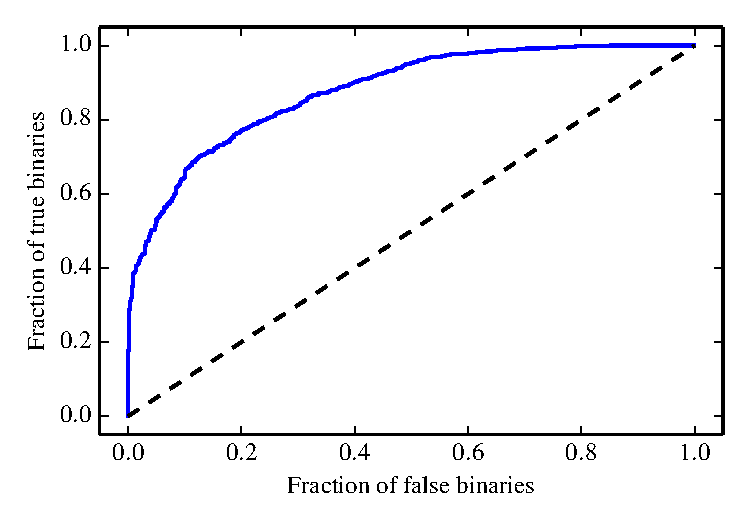
\includegraphics[width=\columnwidth]{ROC_binaries.pdf}
    \caption{Binary ROC plot. \aw{Plot will be ready shortly.}}
    \label{fig:ROC_binaries}
\end{figure}









\section{Conclusions}








\section*{Acknowledgements}

The Acknowledgements section is not numbered. Here you can thank helpful
colleagues, acknowledge funding agencies, telescopes and facilities used etc.
Try to keep it short.

%%%%%%%%%%%%%%%%%%%%%%%%%%%%%%%%%%%%%%%%%%%%%%%%%%

%%%%%%%%%%%%%%%%%%%% REFERENCES %%%%%%%%%%%%%%%%%%

% The best way to enter references is to use BibTeX:

\bibliographystyle{mnras}
\bibliography{refs} % if your bibtex file is called example.bib

%%%%%%%%%%%%%%%%%%%%%%%%%%%%%%%%%%%%%%%%%%%%%%%%%%

%%%%%%%%%%%%%%%%% APPENDICES %%%%%%%%%%%%%%%%%%%%%

\appendix

\section{Some extra material}


%%%%%%%%%%%%%%%%%%%%%%%%%%%%%%%%%%%%%%%%%%%%%%%%%%


% Don't change these lines
\bsp	% typesetting comment
\label{lastpage}
\end{document}

% End of mnras_template.tex